\documentclass{article}%
\usepackage[T1]{fontenc}%
\usepackage[utf8]{inputenc}%
\usepackage{lmodern}%
\usepackage{textcomp}%
\usepackage{lastpage}%
\usepackage[head=40pt,margin=0.5in,bottom=0.6in]{geometry}%
\usepackage{graphicx}%
%
\title{\textbf{Abogado de la familia: “Actas del caso Albán dicen que fue homicidio”}}%
\author{Estefani Brito | esbrito@el{-}nacional.com}%
\date{20/11/2018}%
%
\begin{document}%
\normalsize%
\maketitle%
\textbf{URL: }%
http://www.el{-}nacional.com/noticias/politica/abogado{-}familia{-}actas{-}del{-}caso{-}alban{-}dicen{-}que{-}fue{-}homicidio\_260366\newline%
%
\textbf{Periodico: }%
EN, %
ID: %
260366, %
Seccion: %
Política\newline%
%
\textbf{Palabras Claves: }%
Política\newline%
%
\textbf{Derecho: }%
1.1%
, Otros Derechos: %
1.10, 1.2%
, Sub Derechos: %
1.1.1.3, 1.10.1, 1.2.2%
\newline%
%
\textbf{EP: }%
NO\newline%
\newline%
%
\textbf{\textit{Joel García, integrante de la defensa, luego de revisar el expediente, reiteró que el concejal no se suicidó}}%
\newline%
\newline%
%
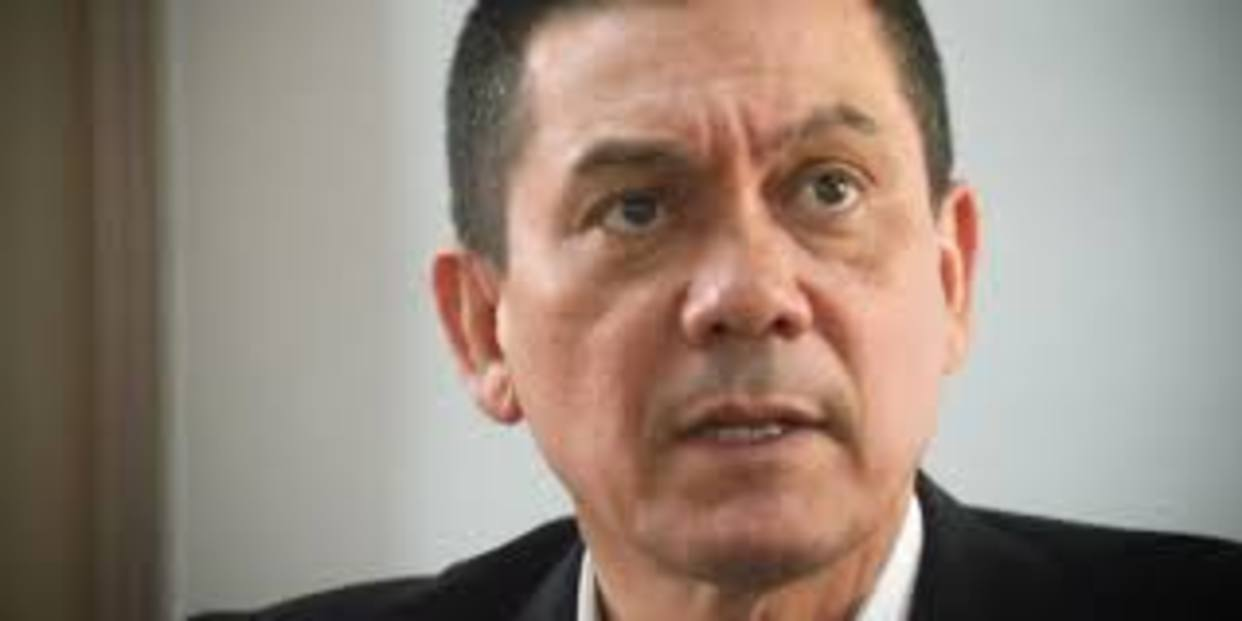
\includegraphics[width=300px]{15.jpg}%
\newline%
%
Joel García, abogado de la familia del concejal Fernando Albán, denunció una vez más irregularidades en la investigación sobre la muerte del edil de Primero Justicia en circunstancias extrañas en la sede del Sebin de Plaza Venezuela%
\newline%
%
Luego de haber revisado el expediente, García destacó que entre esas irregularidades se encuentra el hecho de que las actas, en el folio número 5 correspondiente al inicio de la investigación, colocan homicidio como causa de muerte. Para el abogado esto significa que la fiscal 9° nacional que lleva el caso dice que se trata de un homicidio y no de un suicidio, como ha reiterado el fiscal general designado por la constituyente, Tarek William Saab.%
\newline%
%
“Saab asegura que se trata de un suicidio; si fuese así yo lo invito a que vea el orden de inicio de la investigación que cursa el folio 5 del expediente, en el que la fiscal comisionada coloca como causa de muerte el homicidio”, expresó García en una rueda de prensa, en la que estuvo acompañado por la activista de Derechos Humanos Lilian Tintori, y familiares de presos políticos y caídos.%
\newline%
%
Aseguró que la fiscal 9° nacional pone como causa de muerte el homicidio, basándose en la información que dieron los funcionarios policiales, “los primeros en llegar al lugar”.%
\newline%
%
Señaló que el levantamiento planimétrico que aparece en el folio 155 se observa que en el pasillo del piso 10, donde se encontraba Albán, no hay baños adyacentes, lo que descarta la tesis del Ministerio Público que señala que el concejal solicitó ir a un baño que estaba a escasos tres metros del pasillo y se abalanzó al vacío por una ventana. Descartó que el edil estuviera siendo preparado para su traslado a los tribunales, como asegura la versión oficial, ya que las novedades que aparecen en la página 26, numeral 6, indican que la fiscal a cargo, cuando estaba detenido, Dinora Bustamante, había solicitado que Albán no fuera llevado a los tribunales ese día, sino el martes 9 de octubre; además, las declaraciones de un funcionario de ese órgano policial, señaladas en el folio 83, confirman que “a las 9:00 am ya el Sebin sabía que no iba a trasladar a Albán.%
\newline%
%
Indicó que en las pocas fotos que pudieron verse en el lugar cuando lo rescatan se evidencia que el concejal estaba descalzo. “¿Cómo es que una persona iba a ser traslada sin zapatos al tribunal?”, se preguntó.%
\newline%
%
Resaltó que en las entrevistas que están incluidas en los folios 18, 20, 22, 24, 26, 28, 31 y 33 del expediente, ocho funcionarios del Sebin aseguran que Albán estaba esposado, lo que contradice las declaraciones de Saab que afirma que al momento de su muerte el concejal no las llevaba.%
\newline%
%
Alegó que en el expediente no se evidencian fotos ni videos del antes ni el después de la autopsia que es auditable, como lo asegura Saab. Señaló que los funcionarios del Cicpc que estuvieron presentes junto con otro fiscal en el proceso, afirman que fue practicada por dos personas distintas a las que mencionó la Fiscalía.%
\newline%
%
Aseguró que el cadáver fue removido del sitio donde cayó antes de que llegaran las autoridades competentes, en vez de ser protegido y resguardado como establece la práctica criminalística por lo que no existe ni una solo foto para “establecer de qué manera quedó una vez que supuestamente se lanzó”.%
\newline%
%
Se mostró escéptico de que en el lugar del suceso no hubiera muestra de sangre. “¿Por qué los funcionarios que practicaron la inspección ocular no recabaron ni una gota de sangre en el sitio del ~suceso? Las muestras de sangre las obtuvieron directamente del cadáver, pero no hay recabadas en el lugar del hecho”, dijo.%
\newline%
%
Instó a Saab a inhibirse del caso y exigió que un órgano independiente, imparcial, idóneo, competente y con forense de otros lugares venga a Venezuela a investigar este hecho, por considerar que cualquier investigación que realice el Cicpc o la Fiscalía “siempre llevará a un suicidio”.%
\newline%
%
“El fiscal dijo que todo aquel que asegure que Fernando Albán no se suicidó que lo pruebe; nosotros estamos dando los elementos de convicción para estimar que no se suicidó. Habrá muerto por otras causas. Con toda propiedad, podemos decir que Fernando Albán no se suicidó”, enfatizó.%
\newline%
%
\end{document}